%!TEX root = ../template.tex
%%%%%%%%%%%%%%%%%%%%%%%%%%%%%%%%%%%%%%%%%%%%%%%%%%%%%%%%%%%%%%%%%%%%
%% chapter3.tex
%% NOVA thesis document file
%%
%% Chapter with a short laext tutorial and examples
%%%%%%%%%%%%%%%%%%%%%%%%%%%%%%%%%%%%%%%%%%%%%%%%%%%%%%%%%%%%%%%%%%%%
\chapter{Plano de trabalhos para a Elaboração da dissertação}
\label{cha3}

%This Chapter aims at exemplifying how to do common stuff with \LaTeX. We also show some stuff which is not that common! ;)
%
% https://books.google.pt/books?id=q3DvBQAAQBAJ&pg=PA426&lpg=PA426&dq=APOD+cycle&source=bl&ots=KhoY0esEC7&sig=ecXbOBLk49T0mzgr36h1TJ9XF5I&hl=pt-PT&sa=X&ved=0ahUKEwi6g66pqIXcAhVB46QKHVcbBdkQ6AEIXzAL#v=onepage&q=APOD%20cycle&f=false
\section{Trabalho a desenvolver}
\subsection{Ciclo de desenvolvimento}
Tendo em conta que no decorrer da elaboração não será desenvolvido código de raiz, mas sim optimizar o código existente, através de CUDA ou OpenCL, os esforços a adoptar durante a fase de elaboração seguirão um ciclo de desenvolvimento próprio para programação em GPUs. Este ciclo denomina-se APOD (\textit{Assess}, \textit{Parallelize}, \textit{Optimize}, \textit{Deploy}) \cite{cudaProgGuide} e consiste em quatro fases (figura \ref{apodFig}):
\begin{enumerate}
\item {\textbf{\textit{Assess}}} : Onde é feito um \textit{assessment} ao estado atual do programa, em termos de performance. Nesta fase são determinados os pontos do programa onde este passa mais tempo a executar e identificar os bottlenecks de instruções, através de profilers para confirmar as identificações efectuadas. No caso da dissertação, é feito o profiling do ficheiro bigger.lpi presente na pasta bigger da biblioteca open source para o software que usa o BiGGER, Open-chemera e determinadas as funções que este ficheiro chama onde a fracção de tempo de execução é maior (\textit{hotspots}) assim como zonas de código que atrasam a execução do programa (\textit{bottlenecks}). 

%Pelo que o esforço inicial para a esta etapa do ciclo já se encontra feito. Foram determinados dois pontos paralelizáveis com GPU, a detalhar em \ref{challenges}.
\item{\textbf{\textit{ Parallelize}}} : Após o \textit{assessment}  referido anteriormente estar concluido, procede-se para a fase de implementação do código para paralelizar os pontos encontrados na fase anterior. De acordo com \textit{Six ways to SAXPY}, de Mark Harris  \cite{saxpy}, existem três possibilidades para implementar acelerações: usar bibliotecas aceleradas, diretivas OpenACC ou recorrer a linguagens para programação em GPUs, como CUDA ou OpenCL. Na elaboração da dissertação é pretendido abordar a primeira e terceira possibilidades, no caso da terceira, existe a possibilidade de usar OpenCL pois é suportado pelo IDE Lazarus.

\item{\textbf{\textit{Optimize}}} : Nesta terceira fase é pretendido aumentar a performance da solução base, inicialmente esta ultima tem de ser determinada executando o programa com um dataset de tamanho adequado. Da mesma forma é pretendido recorrer às técnicas descritas na subsecção \ref{optmi} para maximizar a performance assim como às abstrações de outros programas relatados na subsecção \ref{gpus1}.

\item{\textbf{\textit{Deploy}}} : A última fase do ciclo consiste em confrontar a performance obtida com as expectativas fundamentadas no início do ciclo. Se os resultados obtidos não corresponderem ao speedup potencial registado na fase inicial, é necessário voltar à fase \textit{Assess}, recomeçando o ciclo.
\end{enumerate}

     \begin{figure}[ht]
  \centering
    {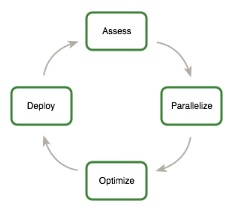
\includegraphics[width=0.5\linewidth]{APOD}}
  \caption{ Diagrama do ciclo de desenvolvimento APOD\cite{cudaProgGuide}.}
  \label{apodFig}
\end{figure}

\subsection {Profiling}
\label{profiling}
%Mudar que não vai ser feito nesta fase o profiling, o programa não assume as condições para que se possa fazer o profiling, justificar que o código tem funções deprecated e houve mesmo erros de compilação. Pelo que a primeira coisa a fazer na elaboração é aplicar atualizar o código, mudando a chamada no ficheiro oclconfiguration.pas sobre de filutuils para LazFileUtils.
De forma a confirmar as assumpções sobre as zonas de código a optimizar para execução na GPU, será necessário fazer uma averiguação sobre o custo de cada etapa do mesmo em termos de número de chamadas e tempo total de computação, através de um profiler. Na tentativa de fazer esta actividade, foi verificado que no código fonte existem chamadas para funções que estão \textit{deprecated} com uma versão actual do Free Pascal, tornado a compilação e o profiling com ferramentas actuais difícil. Neste contexto uma das primeiras tarefas a desempenhar será a actualização do código fonte seguido do profile à performance do BiGGER. O profiling será feito aos ficheiros relacionados com o funcionamento deste último, pois existem elementos do Open-chemera que não são importantes para o mesmo, como por exemplo o ficheiro \textit{chemera.lpi} é o que é necessário compilar e executar no Lazarus para a parte gráfica do Open-Chemera, não influenciando a parte do BiGGER, que é independente. Para executar a componente do BiGGER, é necessário passar como parâmetro um conjunto de ficheiros xml com a informação sobre os átomos das proteínas.  No caso do Lazarus é possível recorrer a duas formas principais para fazer profiling a um programa \cite{lazProf}:
\begin{itemize}
\item gprof : Pode-se utilizar o gprof para fazer profiling em Lazarus, gerando um ficheiro de texto com os dados necessários para averiguar quais as funções do ficheiro bigger.lpi que podem representar oportunidades de paraleliação. 
\item LazProf: IDE de profiling para o Lazarus, que funciona complementada com o FPProfiler. 
\end{itemize}  

 A abordagem LazProfiler requer uma instalação complexa mas é a alternativa cujo profiling mostra os resultados com qualidade superior, sendo necessário apenas ordenar na interface do programa a execução do programa. A alternativa é usar o gprof, que é suportado pelo compilador FreePascal pelo que não requer uma instalação com o nível de complexidade da do LazProfiler, no entanto os resultados que são obtidos não assumem a mesma qualidade deste último.
 
% Foi optado pelo uso do <alternativa> , apresentando-se os resultados na figura. Para a execução do profile foi abordado um cenário de teste representativo, usando um ficheiro .xml com informação dos átomos respetivos às proteínas.  Os resultados apontam que as zonas de código onde o programa passa mais tempo são:
% %\ref{profileRes}
% \begin{itemize}
% \item{\textbf{Zona 1}}: .
%  \item{\textbf{Zona 2}}: .
%    \item{\textbf{Zona 3}}: .
% \end{itemize}
 
 %Concluir com uma aplicação da lei de gustafson barsis assim como com a lei de amdahl \cite{amdahl}
% \textit{Pending Executar o profiling e apresentar resultados (1 Página com uma tabela)}
\subsection{Possibilidades de optimização} % (fold)
\label{abordagem}
A biblioteca \textit{open-source} para docking de proteínas usada no BiGGER, Open-Chemera, encontra-se implementada em Free Pascal (97.6\% do código total)\footnote[11]{É possível obter a biblioteca e o código fonte do BiGGER através do repositório presente no Github \cite{openChemera}. }. O trabalho a realizar na elaboração é focado sobre o package \textit{docking}, mais precisamente às unidades \textit{bogie.pas} e \textit{dockdomains.pas}. O \textit{bogie.pas} consiste no módulo que trata a componente geométrica do docking e na unidade \textit{dockdomains.pas} são determinados os dominios nos três eixos para a simulação da docagem geométrica.

 O trabalho poderá abarcar a paralelização de unidades adicionais presentes no pacote \textit{docking} o que só garante melhorias adicionais à performance da biblioteca Open-Chemera. 
% por exemplo na secção \ref{challenges} é abordada uma paralelização à unidade linegrids.pas, que é a unidade onde é feito o cálculo das regiões de superficie e core dos pares assim como a determinação das grelhas para a superficie 3D dos mesmos, para o efeito de complementar a resolução do desafio distipulado na secção.
% As principais alterações serão, no entanto, focadas nos dois referidos anteriormente.
 
Face à possibilidade de não existir nenhuma versão do CUDA para programar paralelizações em Free Pascal, poderá ser optado por desenvolver as optimizações usando OpenCL, que é suportada pelo Lazarus. Este ultimo é o IDE a utilizar durante o trabalho de elaboração. É possível, no entanto, implementar uma biblioteca acelerada (ficheiro dll) para o BiGGER com CUDA.

%Poderão vir a ser implementados para a paralelização das duas unidades, \textit{kernels} que executam operações de mapeamento, em que o espaço de possibilidades a tratar na primeira fase do BiGGER poderá ser associado a uma estrutura de dados, dividida por blocos em que estes últimos serão constituidos por casas indexadas pelo ID da thread correspondente. Pelo que a indexação geral estará associada a uma fórmula que envolva a posição da thread no bloco e o número de bloco. Para cada uma das posições o core da GPU executará a função que determina se a configuração é aceite ou não.
%Este esquema de indexação de threads também existe em OpenCL, por invocações próprias na sua sintaxe.
%     \begin{figure}[ht]
%  \centering
%(figura \ref{fig:fig3subfig})
%    {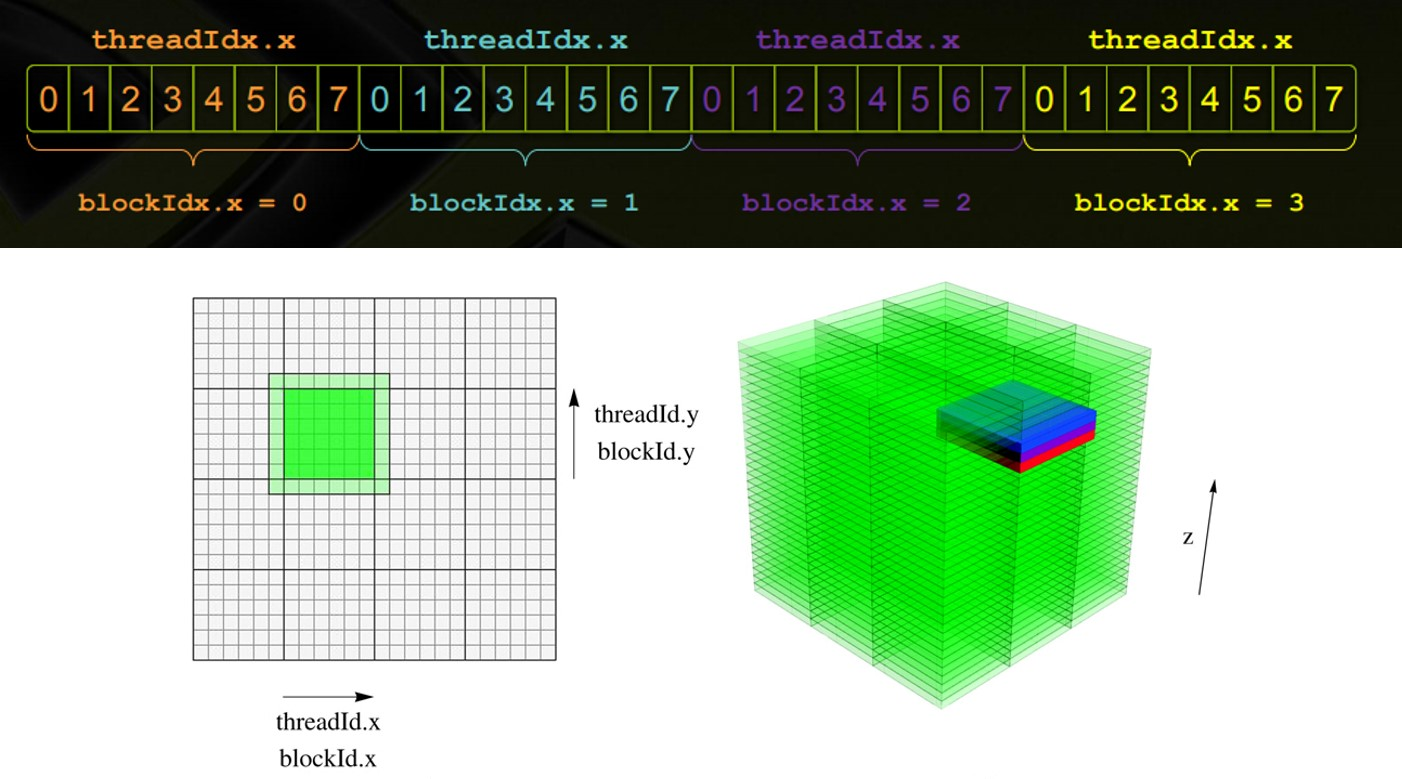
\includegraphics[width=0.5\linewidth]{Imagem1}}
%  \caption{Representação gráfica do ID geral de uma thread num array divido por blocos, em CUDA. Adaptações de \cite{Sainio2010CUDAEASYA} \cite{zeller2011cuda}}
%  \label{fig:fig3subfig}
%\end{figure}

%Confirmar com o profiling
Os pontos de optimização focam-se nos seguintes:
\begin{itemize}
\item{\textbf{Criação das grelhas tri-dimensionais}} : 
%In this step, two new Boolean matrices are generated for
%each docking partner. One—the surface matrix—containing
%a definition of the molecular surface (a hollow shell
%with the protein shape) and the other—the core matrix—
%representing the positions belonging to the inner core of
%the protein.
%More precisely, the surface region is defined as the set of
%volume matrix cells that are occupied by the protein shape
%(i.e., have a value 1) and have at least one neighbor cell
%that is empty (i.e., has a value of 0). Computationally, the
%process of defining the molecular surface is very simple. A
%copy of the volume matrix is shifted one location in each of
%the 26 possible directions at a time, and an Exclusive Or
%(XOR) logical operation is performed between the shifted
%and the original matrices. Since the result of a XOR
%operation is True only if both operands are different, this
%will result in a double surface shell that can be trimmed
%with an And operation with the original volume matrix
%(Fig. 2). At this point, each protein is represented by two
%3D matrices: the surface matrix and the core matrix. This
%type of representation is very economical, since one unique
%bit (0 or 1) is needed to define one surface location and one
%byte may contain 8 surface locations at once. The matrices
%are also encoded in a compact form, taking advantage o
Tal como foi mencionado na subsecção \ref{biggerAlg}, um dos passos iniciais do BiGGER consiste na criação de duas grelhas tri-dimensionais de booleanos, para cada um dos elementos do par, que assumem valor 1 ou 0 se a posição respetiva na grelha corresponde a uma posição atómica da proteina. Neste contexto, é possível determinar a região de superficie de cada proteina, sendo esta definida pelo conjunto de todos os nós da matriz que se encontram a 1. Na versão sequencial do BiGGER, a região de superficie das proteínas é determinada fazendo um \textit{shift} da cópia da grelha uma casa para o lado em cada uma das 26 direções possíveis, aplicando uma operação lógica XOR entre os nós originais e os que foram deslocados. É possível acelerar este procedimento implementando um kernel em que é mapeada a grelha original na GPU e distribuindo cada uma das direções pelos SMs.

%Analisando o código que se pode encontrar na unidade dockdomains.pas pode-se verificar que existem uma certa diversidade nas possibilidades de optimização.  
%
%O código presente nesta unidade contém um conjunto de \textit{procedures} que executam cadeias de ciclos for/while, em teoria é possível paralelizar o dockdomains recorrendo a kernels que executam operações de map, de forma a reduzir a carga de computação.
%
%Paralelizações adicionais poderão ser feitas na unit linegrids.pas que permitem trazer melhorias extra de performance, no entanto serão alterações complementares, segundo a documentação inicial do código fonte da unidade, os segmentos gerados por esta unidade são referenciados apenas ao eixo z, sendo então uma unidade auxiliar para o BiGGER para a indexação da matriz tri-dimensional por parte deste.

%For every relative orientation of the two proteins, the
%translational interaction space is searched by systematically
%shifting the matrices defining one molecule (the
%Probe) relative to the matrices representing the other
%partner (the Target). This movement is performed in
%discrete steps of the size of the matrix cells. The extent of
%surface matching between the two molecules is thus
%simply evaluated by the number of surface cells of the
%target molecule overlapping any surface cells of the probe.
%Computationally, this process is made very fast by applying
%the AND Boolean operator to the memory registries
%containing the two surface matrices. A value of 1 is
%obtained for every position simultaneously occupied by the
%surfaces of both proteins and 0 elsewhere. At the same
%time, every solution that results in overlapping core cells of
%both molecules is immediately discarded, thus rejecting
%solutions involving unrealistic interpenetration of the
%docking partners. However, core-surface overlaps are allowed
%and this represents the second level of “softness” in
%the algorithm.
%Finally, the probe is rotated a certain amount (typically
%15°) relative to the target and this process (digitization,
%translation, surface matching) is repeated until a complete
%non-redundant search in the 6-dimensional space is performed

\item{\textbf{Pesquisa de sobreposições}} : De forma a poder avaliar a correspondência entre as superficies dos pares, para cada rotação a ser tratada é aplicada uma operação de shift, à semelhança do passo anterior, mas desta vez com as matrizes originais de ambos os elementos do par. A determinação de sobreposições é feita determinando o número de sobreposições entre os nós de superficie de ambas as proteínas. Na versão sequencial, para determinar as sobreposições é necessário aplicar uma operação lógica AND entre os registos de memória que contêm as matrizes de superficie. Por sua vez situações em que existam sobreposições entre nós \textit{core} são descartadas como candidatos, no entanto situações em que são sobrepostos um nó \textit{core} com um nó de superficie não são. É feita uma rotação entre os pares de proteínas em um ângulo de 15º por omissão, repetindo os processos de criação das grelhas, translação por shift e correspondência de superficie até todas as possibilidades num espaço de 6 dimensões estarem cobertas. Este procedimento assume as mesmas condições do que a etapa do Megadock correspondente à rotação do ligando, neste o processo para cada átomo (representado como um nó da grelha do ligando) é independente, sendo mapeado para a GPU. Neste contexto é possível abordar uma optimização em que os nós da grelha são mapeados para a GPU. Cada um dos nós serão processados por um core da GPU e o AND passa a ser aplicado entre registos da GPU em vez de ser em registos da CPU.
%During the search procedure, up to 109 different modes
%of contact between two proteins may be assessed (depending
%on the molecular size). It is absolutely necessary to
%drastically reduce this number of putative solutions before
%they can be evaluated according to any energy terms. A
%sub-population of 1,000 binding modes is actually kept,
%which represents a reduction of more than 99.999% of the
%total solutions sampled.
%During this work, two levels of filtering were tested to
%discard unlikely solutions. The simplest one uses the
%unique criterion of geometric complementarity. After each
%evaluation of surface matching, its value is compared with
%a sorted lookup table containing those of the 1,000 best
%matching solutions found so far. If its surface matching is
%poorer than that of the worst solution in the table, then it
%is discarded. Otherwise, it is saved and the geometry of the
%worst element in the table is eliminated.
%As discussed above, pure geometric surface complementarity
%may not be sufficient as the sole criterion to safely
%eliminate unlike binding modes. Within our test cases, we
%found many situations where the native-like complex has a
%poor intermolecular surface contact compared to many
%alternative incorrect solutions. This can cause the nativelike
%solution to be pushed down the table of top scores and
%eventually, in some cases, to be excluded from the table of
%retained solutions.
%Therefore, a more complete and combined criterion is
%used, where indicated, to filter out unlike docked geometries.
%In this procedure, the list of retained solutions is
%still sorted by surface matching score and every solution
%with a lower index of surface matching, than the last
%element in the list, is immediately discarded, as above.
%However, the remaining complexes are not automatically
%kept. They are checked for pairwise amino acid contacts
%across the molecular surface (see Side Chains Interactions
%below) and only those possessing favorable net amino acid
%interactions are then inserted in the list of saved solutions
%and the last element is discarded.
%Since this operation is performed for the very small
%percentage of eligible docked geometries with higher surface
%matching scores, it does not significantly slow the
%search and filtering process.

\item{\textbf{Filtragem de Candidatos}}: O BiGGER contem um passo de filtragem de candidatos, em que $10^{9}$ possíveis contactos entre as proteínas são filtrados, sendo eliminados no final deste processo $99.999\%$ destes. O processo consiste em usar uma combinação de critérios, sendo esta combinação composta inicialmente por complementaridade de superficie, seguida pelo número de contactos favoráveis entre pares de amino-ácidos. A avaliação é determinada para cada candidato e esta é comparada com as avaliações presentes numa tabela com as 1000 melhores encontradas até ao momento. Se a avaliação mostrar que a solução é pior do que a do último elemento da tabela, a solução é descartada. Em caso de ser melhor, a solução é guardada na tabela e o último elemento da lista é descartado. Uma optimização a considerar para este passo será distribuir a computação relacionada com as avaliações da complementaridade de superficie e número de contactos em dois \textit{kernels}. A tabela com os melhores candidatos poderá ser guardada em memória partilhada na GPU, pois é nesta memória que os acessos são mais rápidos do que na memória global. De notar que nesta fase são feitos muitos acessos à tabela para alterar o conteúdo desta, pelo que é importante que estes sejam rápidos.
%At this stage, the four individual interaction terms
%evaluated for each docking solution (either individual or
%cluster) must be properly combined into a global scoring
%function. This will be the criterion used to rank docking
%results and to distinguish the near-native solutions—
%which resembles the experimentally determined structure
%of the complex—from the majority of other incorrect
%solutions.
%None of the interaction terms is sufficient per se to be
%used as a judging criterion. Besides, the theoretical backgrounds
%behind each of the interaction terms are quite
%disparate and they are expressed in different units and
%scales, so they cannot be directly compared. However, the
%main assumption behind the scoring function herein described
%is that a proper combination of the four independently
%calculated interaction terms should include, in one
%way or another, most of the relevant details determining
%the molecular recognition and specificity of non-covalent
%protein complexes.
%The scoring function is empirically defined through a
%learning process using neural network technology and
%aiming at predicting the known crystallographic structures
%of a series of protein complexes.
%The classification system used is a feed forward neural
%network with three hidden layers (with 4, 3, and 2
%neurons, respectively) and a single output neuron. The
%input values for the network are the four interaction terms
%calculated for each solution (or cluster of solutions) and its
%output is a single scoring value, which is an estimate of the
%likelihood of that solution representing a near-correct
%binding mode. In the process of training and testing, each
%docked geometry was labeled as a near-correct solution if
%its RMS deviation (a-carbons) from the crystallographic
%complex was less than 4.0 Å. Otherwise it was labeled as
%incorrect.
%The training phase used a neural network back propagation
%algorithm30 and was targeted at maximizing the
%distinction between near-correct and incorrect structures
\item{\textbf{Scoring}}: Na fase de scoring do BiGGER, são considerados quatro termos individuais na avaliação de cada solução encontrada: complementaridade de superficie, contactos entre ámino-acidos, electroestática e solvatação. Estes quatro termos são combinados numa função de scoring global, sendo esta última calculada para cada um dos candidatos, à semelhança do que é feito para o PIPER sobre os seus conjuntos de quoficientes na função de score. Poderá ser necessário aplicar uma optimização em que os procedimentos associados quatros termos são distribuidos por 4 SMs, pelo que esta optimização poderá ser semelhante à correspondente ao uso do segundo kernel no conjunto de optimizações para o PIPER em 2014.
\end{itemize}
\section{Metodologia de Avaliação}
% o que vais avaliar e como? ou seja quais serão as métricas de sucesso? aqui é fácil será a redução do tempo de execução, mantendo a correção dos resultados
No final de cada iteração do ciclo, serão feitas análises de performance ao BiGGER, onde serão avaliadas ambas redução de tempo de execução e exactidão dos resultados face à versão actual do programa.
A exactidão poderá ser feita submetendo a versão optimizada do BiGGER aos testes aplicados à versão sequencial, procurando coincidencias nos resultados. Por sua vez a redução do tempo de execução poderá ser avaliada comparando os valores de speedup da solução desenvolvida em cada ciclo com o speedup máximo teórico. Segundo o guia de boas práticas da NVIDIA \cite{cudaProgGuide}, os conceitos de escalabilidade forte e fraca são necessários para determinar o quanto um programa pode ser paralelizado. No entanto usar um ou outro depende das características do problema que o programa resolve. É recomendado considerar a escalabilidade forte quando o tamanho do problema é constante e o tempo de solução decresce à medida que o número de processadores aumenta. Em alternativa a escalabilidade fraca é considerada quando o tamanho do problema varia à medida que o número de processadores aumenta. No caso do BiGGER e da modelação das interações entre moléculas, o tamanho destas pode variar com a complexidade da molécula, mas o tamanho é constante no decorrer da execução do programa. Da mesma forma o tamanho das grelhas criadas inicialmente não é variável assim como o número de direções para onde a operação de shift entre as grelhas, pelo que é aplicável a escalabilidade forte a este problema. Neste contexto o speedup máximo teórico pode ser determinado após a fase \textit{Assess} em cada ciclo estar concluida, recorrendo à lei de Amdahl \cite{amdahl1967}, em que o speedup máximo teórico é dado pela fórmula $ S = 1 / ( 1 - P )$, sendo S o speedup máximo teórico que o programa pode alcançar e P a fração sequencial do código que pode ser paralelizado. O speedup corrente, por sua vez, pode ser determinado através da fórmula $S = t1/ tp$, sendo $t1$ o tempo de execução da versão do BiGGER que usa apenas a CPU e $tp$ o mesmo tempo para a versão que usa ambos CPU e GPU.
% section document_structure (end)
\section{Plano de Trabalhos} % (fold)
O plano de trabalhos consistirá em quatro iterações do ciclo APOD, para cada um dos pontos de optimização apresentados na sub-secção \ref{abordagem}, tendo cada um dos ciclos uma carga de horária total de 224 horas de trabalho nos dias úteis (tabela \ref{tabPlano}). Esta carga horária será repartida pelas quatro etapas do ciclo APOD, em que a primeira etapa do ciclo terá uma carga horária de 24 horas, a segunda e terceira etapas 80 e a quarta etapa, que é concorrente com um bloco dedicado à escrita do relatório, tem uma duração de 40 horas. Neste contexto o primeiro ciclo será iniciado quando o ano lectivo iniciar a 10 de Setembro de 2018, em que será feito o trabalho respetivo à fase \textit{Assess}. O programa será submetido a um profiler e serão confirmados os pontos de optimização identificados na fase de preparação da tese. Após a conclusão da fase anterior, é dado início às fases \textit{Parallelize} e \textit{Optimize}, cada uma num bloco de actividade com uma duração de 20 dias úteis de trabalho para ambas as fases. Nestas duas fases serão implementadas as optimizações para os problemas de performance indicados na fase anterior. Na eventualidade de ocorrerem optimizações que ficaram pendentes, o esforço será transferido para os blocos \textit{Parallelize} e \textit{Optimize} da iteração seguinte. O passo final do ciclo, \textit{Deploy}, será acompanhado com a actividade de escrita do relatório. A primeira iteração será terminada a 17 de Outubro de 2018.  \par 
A segunda iteração do ciclo será iniciada dia 18 de Outubro de 2018, onde serão repetidos os procedimentos do ciclo anterior para a segunda versão optimizada do algoritmo, e terminará dia 26 de Novembro de 2018. A terceira iteração terá inicio a 27 de Novembro de 2018, 
A quarta iteração do ciclo será iniciada a 4 de Janeiro de 2019,  terminando em 11 de Fevereiro de 2019, o que garante uma margem de atrasos relacionados com as fases \textit{Optimize} e \textit{Parallelize} de todas as iterações de duas semanas até ao inicio do mês onde será procedida à entrega da dissertação. Na eventualidade de o trabalho de implementação não se encontrar a correr dentro do plano, o espaço de tempo entre o fim da quarta iteração e a data de entrega pode ser adaptado para integrar uma quinta iteração, a decorrer até dia 20 de Março de 2019. No entanto o esforço nesta iteração terá de ser complementado com a elaboração do relatório de dissertação.
 Se o contrário se verificar e o trabalho estiver dentro do prazo, após o final do quarto ciclo de desenvolvimento, será focada a elaboração do relatório de dissertação até à data de entrega deste, que segundo o calendário publicado para o ano lectivo de 2018-2019, é dia 25 de Março de 2019. A fase de elaboração do relatório terá uma carga horária total de 233 horas. Este plano consome na totalidade 1121 horas de trabalho (apenas dias úteis), garantindo aproximadamente 40 ECTS de esforço. No entanto como a elaboração da dissertação será acompanhada com uma unidade curricular pendente, reduzindo a contribuição para 34 ECTS, sendo superior ao 30 ECTS exigidos para a cadeira correspondente à fase de elaboração da tese.
\label{plan}
%   \begin{figure}[ht]
%  \centering
%    {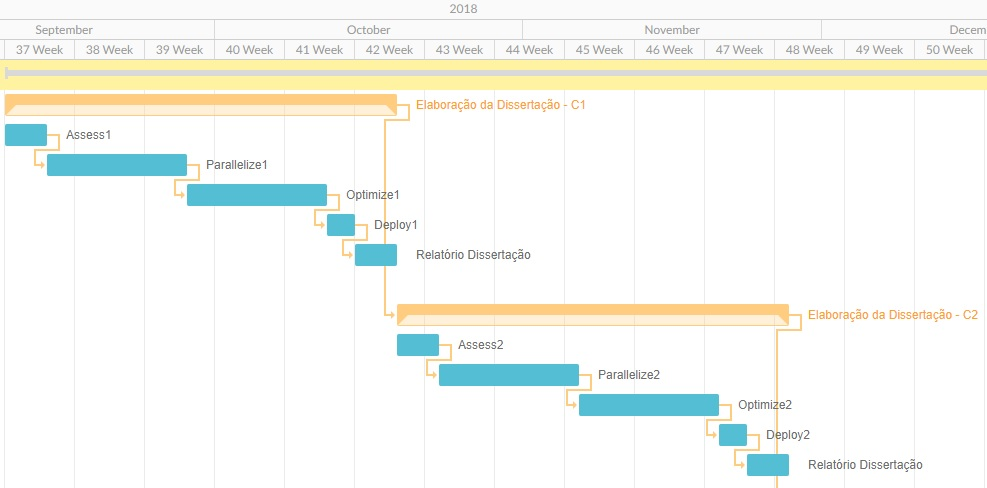
\includegraphics[width=0.75\linewidth]{Plan1}}
%  \caption{ Os primeiros dois ciclos de desenvolvimento, a decorrer entre principio de Setembro e o final do 1º Semestre.}
%  \label{apodFig}
%\end{figure}
%   \begin{figure}[ht]
%  \centering
%    {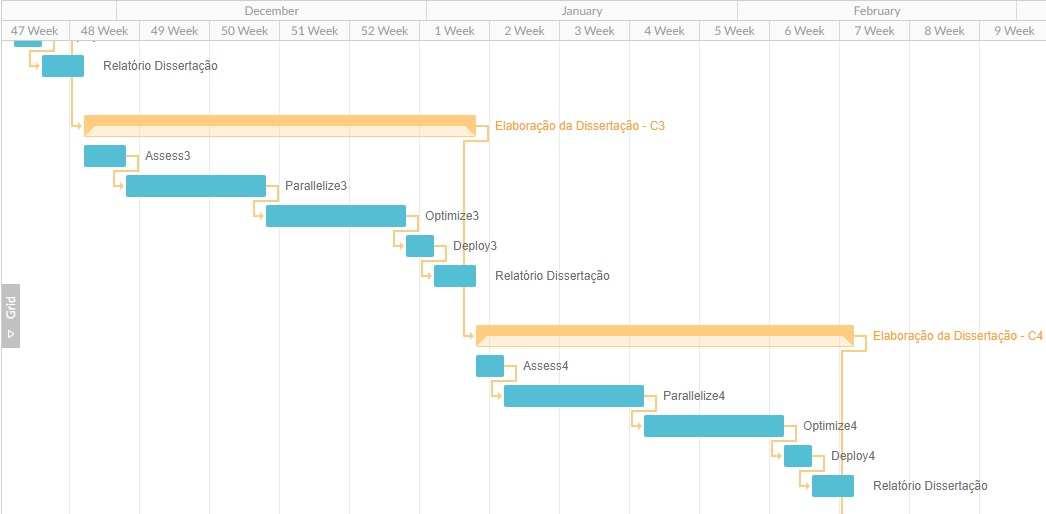
\includegraphics[width=0.75\linewidth]{Plan2}}
%  \caption{Os dois ultimos ciclos de desenvolvimento, a decorrer após o final do 1º até ao final do periodo intercalar.}
%  \label{apodFig}
%\end{figure}
\begin{table}[]
\begin{tabular}{|l|l|l|l|}
\hline
                                 & Inicio              & Fim                 & Carga de trabalho (horas) \\ \hline
\textbf{Iteração 1}              & \textbf{10/9/2018}  & \textbf{17/10/2018} & \textbf{224}              \\ \hline
Assess 1                         & 10/9/2018           & 12/8/2018           & 24                        \\ \hline
Parallelize 1                    & 13/9/2018           & 26/9/2018           & 80                        \\ \hline
Optimize 1                       & 27/9/2018           & 10/10/2018          & 80                        \\ \hline
Deploy e Relatório 1             & 11/10/2018          & 17/10/2018          & 40                        \\ \hline
\textbf{Iteração 2}              & \textbf{18/10/2018} & \textbf{26/11/2018} & \textbf{224}              \\ \hline
Assess 2                         & 18/10/2018          & 22/10/2018          & 24                        \\ \hline
Parallelize 2                    & 23/10/2018          & 5/11/2018           & 80                        \\ \hline
Optimize 2                       & 6/11/2018           & 19/11/2018          & 80                        \\ \hline
Deploy e Relatório 2             & 20/11/2018          & 26/11/2018          & 40                        \\ \hline
\textbf{Iteração 3}              & \textbf{27/11/2018} & \textbf{3/1/2019}   & \textbf{224}              \\ \hline
Assess 3                         & 27/11/2018          & 29/11/2018          & 24                        \\ \hline
Parallelize 3                    & 30/11/2018          & 13/12/2018          & 80                        \\ \hline
Optimize 3                       & 14/12/2018          & 27/12/2018          & 80                        \\ \hline
Deploy e Relatório 3             & 28/12/2018          & 31/12/2018          & 40                        \\ \hline
\textbf{Iteração 4}              & \textbf{4/1/2019}   & \textbf{11/2/2019}  & \textbf{224}              \\ \hline
Assess 4                         & 4/1/2019            & 7/1/2019            & 24                        \\ \hline
Parallelize 4                    & 8/1/2019            & 21/1/2019           & 80                        \\ \hline
Optimize 4                       & 22/1/2019           & 4/2/2019            & 80                        \\ \hline
Deploy e Relatório 4             & 5/2/2019            & 11/2/2019           & 40                        \\ \hline
\textbf{Elaboração do relatório} & \textbf{12/2/2019}  & \textbf{25/3/2019}  & \textbf{233}              \\ \hline
\end{tabular}
\caption{Tabela cronograma do plano de trabalho.}
\label{tabPlano}
\end{table}

\section{Profiling na fase Inicial}
Nesta fase inicial foi feita uma análise de performance ao BiGGER na versão sequêncial conforme foi indicado no plano de trabalhos na fase de preparação. Como tal a biblioteca open-chemera foi submetida a um conjunto extenso de testes a variar parametros específicos como o nº de átomos do ligando/receptor, a sobreposição mínima das superfícies moleculares e o nº de rotações no docking como está indicado na tabela. A ferramenta usada para a actividade foi a única que funcionou de diversas alternativas que podem ser usadas para fazer profiling a um programa que se encontra em FreePascal - Valgrind/Callgrind. Este programa devolve resultados que incluem o número total de chamadas efectuadas para uma dada função e duas métricas de avaliação de custo temporal: self cost e inclusive cost. Para efeitos de amostragem de resultados, foi considerada principalmente o self cost pois este refere-se à fração de tempo de execução que é passado dentro da função.
%PENDING : POR A TABELA QUANDO TIVER INTERNET
\subsection{Sobre os parametros de teste}
\subsubsection{Complexos de proteínas usados}
Para que seja possível determinar o impacto do formato dos pares na performance do BiGGER, apenas foram considerados pares ligando-receptor que assumam formatos uniformes, sendo considerados apenas cubos e esferas para os testes. Adicionalmente, não foram testadas situações em que, por exemplo, o ligando tem forma cubica e o receptor esferica, pois isto implica duplicar a quantidade de testes necessários. Em termos de número de átomos, não foram aplicados testes em que o número de átomos do receptor seja menor do que  o número de átomos do ligando. Este cenário não corresponde a uma situação real assim como introduz esforços adicionais ao BiGGER que são desnecessários. Conforme foi referido no capítulo \ref{cap2} o BiGGER resolve o problema de docking através de um conjunto de passos, entre eles a digitização de grelhas tridimensionais. É criada e digitizada uma vez a grelha do receptor e tantas vezes como rotações pedidas a grelha do ligando.
\subsubsection{Sobreposição mínima e rotações}
Foi pretendido estudar o impacto da variação da sobreposição minima na fase de scoring do algoritmo, sendo que esta foi incrementada de forma gradual entre o valor nulo e um valor excessivamente grande para uma situação real. Sobre as rotações, foi aplicado o mesmo procedimento utilizado na sobreposição mínima, neste caso o número de rotações foi variado gradualmente entre 100 rotações, valor baixo para uma situação real e 6000/15000, sendo que estes últimos são usados habitualmente num docking.

\subsection{Scripts desenvolvidos para a fase de profiling}
Tendo em conta as variações de parametros referidas na tabela x, o leitor fica remetido para a extensão de cenários de teste possíveis de realizar, produto do nº de combinações possíveis. No total foram realizados x testes, em que para cada um foram necessários aplicar passos manuais como:
\begin{enumerate}
	\item{A criação através do elemento dockprep do BiGGER do ficheiro de job (xml) para o docking, sendo este último completado pela execução do BiGGER.}
	\item{Alteração dos campos necessários do ficheiro xml para o docking estar dentro do cenário pretendido. }
	\item{Executar o teste por linha de comandos}
	\item{Guardar os resultados numa folha excel}
\end{enumerate} 
Todo este processo para cada um dos x testes fez com que o processo de realizar o profile ao BiGGER tenha demorado excessivamente. Como tal foram implementados 3 scripts que automatizam/ facilitam o procedimento, também diminuem a probabilidade de erro humano na execução do último passo do procedimento. O primeiro script, em python, automatiza os dois primeiros passos do procedimento. O programa recebe como input um conjunto de argumentos que descrevem o cenário pretendido, e cria como output um ficheiro xml de job com o mesmo formato dos criados pelo dockprep para a execução do BiGGER completar, mas com os parametros alterados. Os argumentos deverão ser indicados pela ordem referida:
\begin{enumerate}
	\item{a}
	\item{b}
	\item{c}
	\item{d}
\end{enumerate} 
O segundo script é um ficheiro com uma sequência de comandos para um terminal linux. O terceiro programa que similarmente ao primeiro foi desenvolvido em python cria gráficos lineares com os valores de self cost obtidos pelo callgrind para o conjunto de funções mais problemáticas no open-chemera, através da letura de uma matriz com estes valores, gerando três agrupamentos. Um contem apenas os gráficos em que foi variado apenas o numero de átomos presentes no ligando e no receptor, um segundo onde os gráficos variam só a sobreposição e um último onde é variada apenas a rotação. O output do script pode ser observado nas figuras x, y, e z.
Estes scripts automatizam a grande maioria do workflow necessário para aplicar o profilling. Falta no entanto automatizar introdução/ actualização dos valores de self cost na matriz de onde são gerados os gráficos que neste momento não é possível de concretizar. 

\subsection{Conclusões}
Após a análise dos dados obtidos nesta fase inicial, foram tiradas algumas conclusões. Verificou-se que existem problemas de performance nas unidades partilhadas do open-chemera que este usa para resolver os dockings, mais precisamente as unidades geomhash.pas, na função isInnerPoint e geomutils.pas, na função de distancia euclidiana.
Dos resultados do profiling, é possível inferir:
\begin{enumerate}
	\item{O tempo de execução gasto nas funções das unidades geomhash e geomutils ocupam a maioria ou até mesmo a totalidade do tempo gasto na fase de digitização. Sendo que este tempo cresce à medida que o número de rotações e o tamanho das estruturas aumenta. Neste contexto pode ser inferido que estes parametros têm peso na fase de digitização, que por sua vez ocupa a maior parte do tempo de execução do algoritmo. Pelo que é necessário paralelizar as funções isInnerPoint e distance}
	\item{Pelos gráficos em que é variado o minOverlap, é possível observar que a curva mantem-se constante para a maior parte das situações, variando apenas a curva respetiva à função addModel, em que para um minOverlap nulo os valores de self cost associados a esta função têm valores superiores aos restantes valores de minOverlap. Neste contexto a curva assume-se como descrescente em relação ao self-cost. Este comportamento da curva é justificável pois para valores de minOverlap baixo, o BiGGER pode passar uma parcela de tempo considerável a preencher uma lista de modelos solução com soluções de poses em que o valor de score associado à sobreposição é maior ou igual a 0 até preencher por completo a lista. Se a sobreposição minima for aumentada, a probabilidade do algoritmo encontrar soluções adequadas para reservar na lista baixa, sendo que a lista já não é preenchida e o self cost da função add model baixa, encontrando-se nulo em situações onde o minOverlap têm o valor máximo establecido para a bateria de testes. Como tal infere-se que o parametro sobreposição minima tem peso apenas para a fase de scoring do algoritmo e não para a fase de digitização, por consequência, a paralelização da função addModel passa a ser um objetivo secundário do plano de trabalhos. }
	\item{Existe ainda a função setExtremes da unidade dockdomains, cujos valores de self cost registados não são tão consideráveis como os valores das funções referidas nos pontos anteriores. A paralelização desta função constitui, à semelhança da função addModel, um objetivo secundário. Sobre os valores de self cost, acrescenta-se que as curvas do setExtremes nos gráficos são constantes em todos os gráficos nos 3 agrupamentos, pelo que o comportamento desta função não é afectada por nenhum dos parametros. No entanto é possível notar a diferença dos valores de self cost nos testes em que foram usados complexos com formato cúbico para os com formato esférico. Deste modo conclui-se que é o formato dos complexos que afecta esta função. }
	\item{Este último ponto diz respeito aos limites máximos de valores de self cost associados às funções referidas que podem ser observados nos resultados. Para os cenários de teste mais exigentes verificou-se que o self cost do BiGGER (fração de tempo gasto na execução do bigger) encontrava-se a 96\% e os restantes 4\% dizem respeito às bibliotecas externas auxiliares, sendo que esta fracção de tempo não pode exceder ou alcançar os 100\%. Com base neste facto e na análise dos gráficos gerados, é possível estimar a assimptota horizontal das curvas associadas às funções de distancia e isInnerPoint, que está situada entre os 40\% e 45\% para a primeira e 35\% e 40\% para a última. Esta inferência poderia ser comprovada introduzindo cenários de teste que excedem a exigência máximo considerada para esta fase (aumentar o tamanho dos pares e mais rotações, com overlap minimo nulo), certamente haveria um resultado em que a fração do BiGGER alcançasse os 99\%. No entanto para os cenários actuais mais exigentes, o tempo de execução de cada um demorou 8 horas a executar, o que faz com que executar um teste ainda mais exigente possa demorar até 24H a terminar, não sendo compensável face à alternativa de estimar os limites.  }
\end{enumerate}
%1 de Setembro a 30 Setembro: Familiarização com o código do BiGGER presente no Open-Chemera inclusive profiling caso nao tenha conseguido
% 1ª Semana de Outubro (1 a 6)
% 
%No final de cada ciclo fazer no minimo duas páginas do documento de dissertação com as conclusões.
%1 de Setembro a 30 Setembro: Familiarização com o código do BiGGER presente no Open-Chemera
%\textit{Gantt chart?}
% section dealing_with_bibliogrpahy (end)


%\section{Inserting Tables} % (fold)
%\label{sec:inserting_tables}
%
%% section inserting_tables (end)
%
%
%\section{Importing Images} % (fold)
%\label{sec:importing_images}

% section importing_images (end)


%\section{Floats, Figures and Captions} % (fold)
%\label{sec:floats_figures_and_captions}

% \subsection{Inserting Figures Wrapped with text} % (fold)
% \label{ssec:inserting_images_wrapped_with_text}
% 
% You should only use this feature is \emph{really} necessary. This means, you have a very small image, that will look lonely just with text above and below.
% 
% In this case, you must use the \verb!wrapfiure! package.  To use \verb!wrapfig!, you must first add this to the preamble:
% 
% \begin{wrapfigure}{l}{2.5cm}
%   \centering
%     
\includegraphics[width=2cm]{snowman-vectorial}
%   \caption{A snow-man}
% \end{wrapfigure}	
% 
% \noindent\verb!\usepackage{wrapfig}!\\
% This then gives you access to:\\
% \verb!\begin{wrapfigure}[lineheight]{alignment}{width}!\\
% Alignment can normally be either ``l'' for left, or ``r'' for right. Lowercase ``l'' or ``r'' forces the figure to start precisely where specified (and may cause it to run over page breaks), while capital ``L'' or ``R'' allows the figure to float. If you defined your document as twosided, the alignment can also be ``i'' for inside or ``o'' for outside, as well as ``I'' or ``O''. The width is obviously the width of the figure. The example above was introduced with:
% \lstset{language=TeX, morekeywords={\begin,\includegraphics,\caption}, caption=Wrapfig Example, label=lst:latex_example}
% \begin{lstlisting}
% 	\begin{wrapfigure}{l}{2.5cm}
% 	  \centering
% 	    
\includegraphics[width=2cm]{snowman-vectorial}
% 	  \caption{A snow-man}
% 	\end{wrapfigure}	
% \end{lstlisting}

% subsection inserting_images_wrapped_with_text (end)

% section floats_figures_and_captions (end)

%\lipsum[1-3]
%
%\begin{figure}[htbp]
%  \centering
%  \subcaptionbox{One sub-figure\label{fig:leftsubfig}}%
%    {
\includegraphics[width=0.5\linewidth]{knitting-vectorial}}%
%  \subcaptionbox{Another sub-figure\label{fig:rightsubfig}}%
%    {
\includegraphics[width=0.5\linewidth]{knitting-vectorial}}%
%  \caption{A figure with two sub-figures!}
%  \label{fig:fig2subfig}
%\end{figure}
%
%\textbf{And this is a small text that references the Figure~\ref{fig:fig2subfig} and its Subfigures~\ref{fig:leftsubfig} and~\ref{fig:rightsubfig}.}
%
%\lipsum[1-3]


%\section{Text Formatting} % (fold)
%\label{sec:text_formatting}

% section text_formatting (end)


%\section{Generating PDFs from \LaTeX} % (fold)
%\label{sec:generating_pdfs_from_latex}
%
%\subsection{Generating PDFs with pdflatex} % (fold)
%\label{ssec:generating_pdfs_with_pdflatex}
%
%You may create PDF files either by using \verb!latex! to generate a DVI file, and then use one of the many DVI-2-PDF converters, such as \verb!dvipdfm!.
%
%Alternatively, you may use \verb!pdflatex!, which will immediately generate a PDF with no intermediate DVI or PS files. In some systems, such as Apple, PDF is already the default format for \LaTeX. I strongly recommend you to use this approach, unless you have a very good argument to go for \verb!latex! + \verb!dvipdfm!.
%
%A typical pass for a document with figures, cross-references and a bibliography would be:
%\begin{verbatim}
%$ pdflatex template
%$ bibtex template
%$ pdflatex template
%$ pdflatex template
%\end{verbatim}
%You will notice that there is a new PDF file in the working directory called \verb!template.pdf!. Simple :)
%
%Please note that, to be sure all table of contents, cross-references and bibliographic citations are up-to-date, you must run \verb!latex! once, then \verb!bibtex!, and then \verb!latex! twice.
%% section generating_pdfs_with_pdflatex (end)
%
%\subsection{Dealing with Images} % (fold)
%\label{sub:dealing_with_images}
%
%You may process the same source files with both \verb!latex! or \verb!pdflatex!. But, if your text include images, you must be careful. \verb!latex! and \verb!pdflatex! accept images in different (exclusive) formats.  For \verb!latex! you may use EPS ou PS figures. For \verb!pdflatex! you may use JPG, PNG or PDF figures.  I strongly recommend you to use PDF figures in vectorial format (do not use bitmap images unless you have no other choice).
%% subsection dealing_with_images (end)


%\subsection{Creating Source Files Compatible with both latex and pdflatex} % (fold)
%\label{ssec:creating_source_files_compatible_with_both_latex_and_pdflatex}
%
%Do not include the extension of the file in the \verb!\includegraphics! command. E.g., use\\
%\verb!\includegraphics{sonwman}!\\
%and not\\
%\verb!\includegraphics{sonwman.eps}!.\\
%If you use the first form, \verb!latex! or \verb!pdflatex! will add an appropriate file extension.
%
%This means that, if you plan to use only \verb!pdflatex!, you need only to keep (preferably) a PDF version of all the images. If you plan to use also \verb!latex!, then you also need an EPS version of each image.
%% subsection creating_source_files_compatible_with_both_latex_and_pdflatex (end)
%
%% section generating_pdfs_from_latex (end)


%\newpage
%
%{\Large To be included in the sections above}\\
%
%Para fazer citações, deverá usar-se a chave da referência no ficheiro BibTeX. Se for uma única referência~\cite{Artho04}, usar um ``\verb!~!'' para ligar o \verb!\cite{...}! à palavra que o precede (\ldots\verb!referência~\cite{Artho04}!).  Caso queira fazer múltiplas citações~\cite{Shavit95,Silberschatz06,Moss85}, deverá agrupá-las dentro de um úinico \verb!\cite{...}!.
%
%Note que o ficheiro de bibliografia pode ter tantas entradas quantas quiser. Apenas aquelas cuja chave seja referenciada no texto é que serão incluidas na listagem de bibliografia.
%
%
%Footnotes\footnote{This is a simple footnote.} will be numbered and shown in the bottom of the page.
%
%
%A Tabela~\ref{tab:hla:results} ilustra alguns conceitos importantes associados à contrução de tabelas:
%\begin{asparaenum}[i)]
%	\item Não usar linhas verticais;
%	\item A legenda deve ficar por cima da tabela;
%	\item Usar as macros \verb!\toprule!, \verb!\midrule! e \verb!\bottomrule! para fazer a linha horizontal superior, interiores e inferior, respectivamente.
%\end{asparaenum}
% 
%\begin{table}[ht]
%	\caption{Test results summary.}
%	\label{tab:hla:results}
%\centering
%\begin{tabular}{lccccc}
%	\toprule
%	\multicolumn{1}{c}{\textbf{Test}} 	& \textbf{Anomalies}	& \textbf{Warnings}	& \textbf{Correct} 	& \textbf{Categories}		& \textbf{Missed} \\
%	\midrule
%\cite{Beckman08}~Connection 	& 2 & 2	& 1	& \emph{C}				& 1 \\
%\cite{Artho03}~Coordinates'03 	& 1	& 4	& 1	& \emph{2B, 1C}			& 0 \\
%\cite{Artho03}~Local Variable	& 1	& 2	& 1	& \emph{A}				& 0 \\
%\cite{Artho03}~NASA				& 1	& 1	& 1	& ---					& 0 \\
%\cite{Artho04}~Coordinates'04	& 1	& 4	& 1	& \emph{3C}				& 0 \\
%\cite{Artho04}~Buffer			& 0	& 7	& 0	& \emph{2A, 1B, 2C, 2D}	& 0 \\
%\cite{Artho04}~Double-Check		& 0	& 2	& 0	& \emph{1A, 1B}			& 0 \\
%\cite{Flanagan04}~StringBuffer	& 1	& 0	& 0	& ---					& 1 \\
%\cite{Praun03}~Account			& 1	& 1	& 1	& ---					& 0 \\
%\cite{Praun03}~Jigsaw			& 1	& 2	& 1	& \emph{C}				& 0 \\
%\cite{Praun03}~Over-reporting	& 0	& 2	& 0	& \emph{1A, 1C}			& 0 \\
%\cite{Praun03}~Under-reporting	& 1	& 1	& 1	& ---					& 0 \\
%\cite{IBM-Rep}~Allocate Vector	& 1	& 2	& 1	& \emph{C}				& 0 \\
%Knight Moves					& 1	& 3	& 1	& \emph{2B}				& 0 \\
%	\midrule
%	\textbf{Total}			& \textbf{12}		& \textbf{33}		& \textbf{10}			& \textbf{5A, 6B, 10C, 2D}	& \textbf{2} \\
%	\bottomrule
%\end{tabular}
%\end{table}
%
%
%As figuras a inserir no documento deverão ser de qualidade, preferencialmente em formato vectorial (PDF vectorial) e não em \emph{bitmap} (PNG, JPG, etc). As imagens \emph{bitmap} (Figura~\ref{fig:Figuras_Tree_silhouettes-bitmap}) não escalam bem e têm reflexos negativos na qualidade do seu docuemnto.  Pelo contrário, as imagens \emph{vectoriais} {Figura~\ref{fig:Figuras_Tree_silhouettes-vectorial}} escalam muito tanto quanto o necessário sem degradar a qualidade da imagem.
%
%Só deve usar \emph{screenshots} se não tive mesmo nenhuma alternativa.  Em vez e gerar um \emph{screenshot}, tente usar uma impressora virtual PDF e imprimir para um ficheiro PDF. Regra geral obterá um PDF vetorial. Mesmo que o seu PDF contenha imagens, elas terão sempre qualidade maior ou igual à que obteria com um \emph{screenshot}.
%
%
%\begin{figure}[htbp]
%	\centering
%	
\includegraphics[height=1in]{snowman-bitmap}
%	
\includegraphics[height=3in]{snowman-bitmap}
%	
\includegraphics[height=6in]{snowman-bitmap}
%	\caption{Imagem em formato \emph{bitmap} (JPG)}
%	\label{fig:Figuras_Tree_silhouettes-bitmap}
%\end{figure}
%
%\begin{figure}[htbp]
%	\centering
%	
\includegraphics[height=1in]{snowman-vectorial}
%	
\includegraphics[height=3in]{snowman-vectorial}
%	
\includegraphics[height=6in]{snowman-vectorial}
%	\caption{Imagem em formato PDF vectorial}
%	\label{fig:Figuras_Tree_silhouettes-vectorial}
%\end{figure}
%
%Para agregar várias figuras numa única… Poderá assim referenciar o conjunto~\ref{fig:figura-completa}, a priemira delas~\ref{fig:novelo} ou a segunda~\ref{fig:nuvem}.
%
%
%\begin{figure}[htbp]
%	\centering
%    \subbottom[Novelo de lã] {%
%		\label{fig:novelo}
%		
\includegraphics[height=1in]{knitting-vectorial}
%    }
%\qquad\qquad
%    \subbottom[Tempestade com neve] {%
%		\label{fig:nuvem}
%		
\includegraphics[height=1in]{snowstorm-vectorial}
%    }
%  \caption{Exemplo de utilização de \emph{subbottom}}
%  \label{fig:figura-completa}
%\end{figure}
%
%
%Para incluir listagens de código no seu documento, deverá incluir o pacote \emph{listings} e depois usar o ambiente \emph{lstlisting}, como exemplificado na Listagem~\ref{lst:HelloWorld}.
%
%\lstset{language=Java, caption=Hello World, label=lst:HelloWorld}
%\begin{lstlisting}
%/** 
% * The HelloWorldApp class implements an application that
% * simply prints "Hello World!" to standard output.
% */
%class HelloWorldApp {%
%    public static void main(String[] args) {%
%        System.out.println("Hello World!"); // Display the string.
%    }
%}
%\end{lstlisting}
%
%\section{Equações}
%
%O LaTeX é uma ferramenta poderosa para escrever em estilo matemático. Permite inserir fórmulas no meio do texto como por exemplo esta: $ax^2 + bx + c = 0$. Também permite que as fórmulas sejam destacadas numa linha separada e centradas na página 
%$$x = \frac{-b \pm \sqrt{b^2-4ac}}{2a}$$
%\[x = \frac{-b \pm \sqrt{b^2-4ac}}{2a}\]
%ou numeradas 
%\begin{equation}
%aaa
%\label{eq:1}
%\end{equation}
%que depois pode ser referida no texto como sendo a equação~\ref{eq:1}
%$$\begin{array}{l}
%aa
%\end{array}
%$$
%
%\begin{eqnarray}
%a\\
%b\\
%c\\
%\end{eqnarray}
